\section{Tema 4. Medidas de tensiones, intensidades y resistencias.}
\subsection{Métodos industriales frente a métodos de laboratorio.}
\begin{itemize}
	\item \textbf{Métodos industriales:}
	\begin{itemize}
		\item Utilizan aparatos de medida básicos.
		\item No es necesaria formación especial.
		\item No son muy exactos, pero tienen precisión suficiente.
		\item Dan respuestas inmediatas.
	\end{itemize}
	\item \textbf{Métodos de laboratorio:}
	\begin{itemize}
		\item Requieren equipos de gran calidad metrológica.
		\item Los operadores deben ser capacitados para su uso.
		\item Las tomas de datos se realizan bajo condiciones controladas.
		\item Buscan minimizar la incertidumbre de medida.
	\end{itemize}
\end{itemize}


\subsection{Métodos industriales para medir tensión e intensidad.}
Para un buen resultado se debe prestar atención a:
\begin{itemize}
	\item La selección adecuada de los campos de medida.
	\item La clase del aparato y su error de inserción.
	\item Si el aparato mide el verdadero valor eficaz.
	\item La posición de empleo.
	\item Las condiciones ambientales.
	\item El ancho de banda.
\end{itemize}
\subsection{Error de inserción.}
Debido a la resistencia interna de los aparatos un voltímetro indica una tensión menor a la medida y el amperímetro una corriente menor a la medida. Como los circuitos equivalentes de un voltímetro y amperímetro son:

\begin{itemize}
	\item En voltímetros:
	\begin{itemize}
		\item Es importante que $R << R_V$
	\end{itemize}
	\item En amperímetros:
	\begin{itemize}
		\item Es importante que $R_A << R$
	\end{itemize}
\end{itemize}


\begin{figure}[H]
	\begin{minipage}{0.5\textwidth}
		\begin{figure}[H]
			\centering
			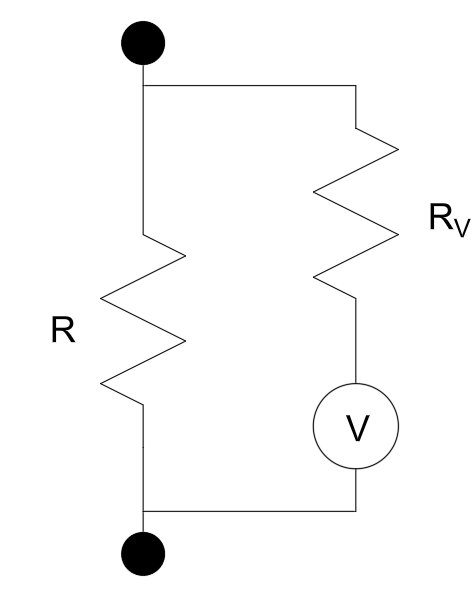
\includegraphics[width=0.7\linewidth]{ImagenesTema4/1}
			\label{fig:1}
		\end{figure}
	\end{minipage}
	\begin{minipage}{0.5\textwidth}
		\begin{figure}[H]
			\centering
			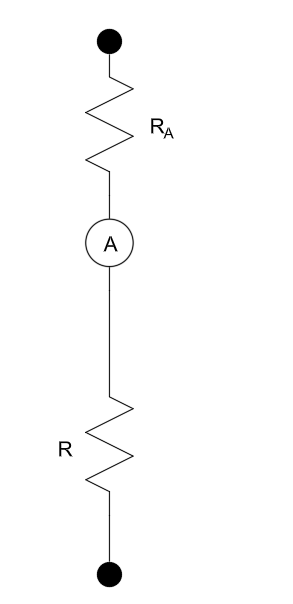
\includegraphics[width=0.7\linewidth]{ImagenesTema4/2}
			\label{fig:2}
		\end{figure}
	\end{minipage}
\end{figure}

\subsubsection{Medida de tensión en circuitos de alta impedancia.}
La conexión de un voltímetro a un circuito de alta impedancia puede producir una reducción importante en la tensión a medir. Para ello, se realiza la siguiente comprobación:

\begin{enumerate}
	\item Se mide la tensión deseada con un voltímetro $U_1$.
	\item Se coloca una resistencia ajustable $R_s$ en serie con el voltímetro y se ajusta hasta que el voltímetro indica una tensión $U_2=\frac{U_1}{2}$.
	\item En función de los valores obtenidos se pueden obtener 2 conclusiones:
	\begin{enumerate}
		\item Si el valor de $R_s$ es igual a $R_V$ la medida no se ve afectada por la inserción del voltímetro.
		\item Si el valor de $R_s$ es mayor a $R_V$ existe efecto de carga y se realiza la siguiente corrección:
		\[U=U_1\frac{R_s}{R_V}\]   
	\end{enumerate}
\end{enumerate}


\subsection{Medida de resistencia con óhmetros.}
\subsubsection{Digitales.}
Su lectura directa es el valor de la resistencia desconocida. Si ese valor es muy reducido, para mejorar el resultado debe restarse la lectura del óhmetro al cortocircuitar los terminales.  El campo de medida elegido debe ser el más próximo al
valor de la resistencia, para que la incertidumbre del
aparato sea mínima y la lectura tenga suficiente resolución.
\subsubsection{Analógicos.}
Hay que hacer un ajuste de cero inicial y cambiar de campo
para que la aguja quede siempre lo más próxima al centro
de la escala (no es lineal).
\begin{figure}[H]
	\centering
	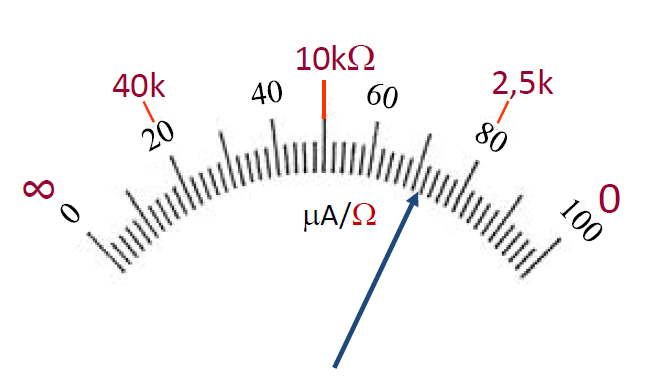
\includegraphics[width=0.5\linewidth]{ImagenesTema4/3}
	\label{fig:3}
\end{figure}



Cabe destacar como la mayor sensibilidad se obtiene cuando la resistencia es nula o igual a la resistencia interna del aparato. Por ello, es mejor medir en la primera mitad de la escala.
\subsection{Medida de resistencia con voltímetro y amperímetro.}
Se mide la corriente y tensión de una carga para obtener la resistencia mediante la ley de Ohm.
\begin{figure}[H]
	\centering
	\label{fig:4}
	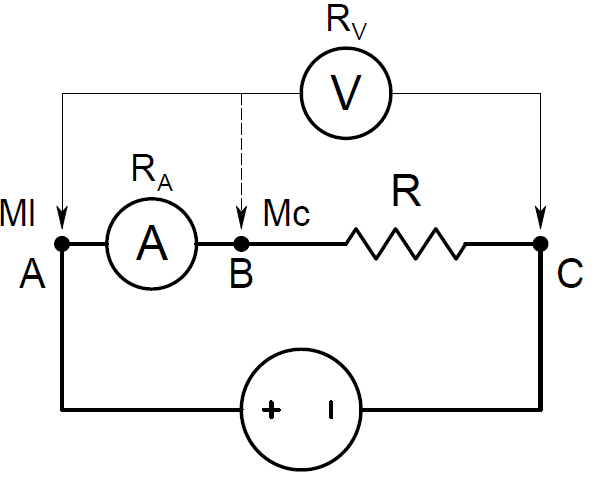
\includegraphics[width=0.7\linewidth]{ImagenesTema4/4}
\end{figure}

En el montaje largo:
\[R'=\frac{U_{AC}}{I_A}=R+R_A\]
\[\epsilon_{ml}=R'-R=R_A \rightarrow \epsilon_{ml(pu)}=\frac{R_A}{R}\]

En el montaje corto:
\[R''=\frac{U_{BC}}{I_A}=\frac{R\cdot R_V}{R+R_V}\]
\[\epsilon_{mc}=-\frac{R^2}{R+R_V} \rightarrow \epsilon_{mc(pu)}=-\frac{R}{R+R_V}\approx-\frac{R}{R_V}\]

Por tanto, para elegir un montaje u otro se igualan los errores y se obtiene el valor crítico:
\[\epsilon_{ml}=\epsilon_{mc}\rightarrow \frac{R_A}{R}\approx\frac{R}{R_V}\rightarrow R_C\approx\sqrt{R_A\cdot R_V}\]
Donde si la resistencia R es mayor a $R_C$ se debe usar el montaje largo y el montaje corto en caso contrario.
\subsection{Medida de R con una $R_p$.}
\subsubsection{Por comparación de corrientes.}
Se mantiene constante $U_0$ se compara la corriente que circula por la resistencia desconocida y la resistencia patrón.
\begin{figure}[H]
	\begin{minipage}{0.5\textwidth}
		\begin{figure}[H]
			\centering
			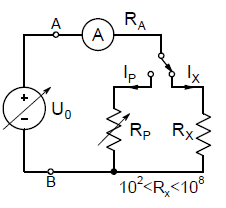
\includegraphics[width=0.7\linewidth]{ImagenesTema4/5}
			\label{fig:5}
		\end{figure}
	\end{minipage}
	\begin{minipage}{0.5\textwidth}
	\[U_0=I_x(R_x+R_A)\]
	\end{minipage}
\end{figure}



\subsubsection{Por comparación de tensiones.}
\subsection{Métodos de laboratorio para medir tensión e intensidad.}
\subsection{Puente de Wheatstone para medida de resistencia.}
\subsection{Puente de Kelvin-Thomson.}